\documentclass[12pt]{article}

\usepackage{amsmath}
\usepackage{unicode-math}
\usepackage{xltxtra}
\usepackage{xgreek}

\setmainfont{Liberation Serif}

\usepackage{tabularx}

\usepackage[table]{xcolor}
\usepackage{tikz}
\pagestyle{empty}

\usepackage{geometry}
 \geometry{a4paper, total={190mm,275mm}, left=10mm, top=10mm}

 \usepackage{graphicx}
 \graphicspath{ {images/} }

 \usepackage{wrapfig}
\usepackage{lipsum}%% a garbage package you don't need except to create examples.

\begin{document}
\part*{\centering{Πανελλήνιες Μαθηματικά Γ Λυκείου 2017 Λύσεις}}

\section*{Θέμα Β}
  \begin{enumerate}
    \item [B1.] Θα πρέπει $x\in A_g$ και $g(x)\in A_f$, δηλαδή $x\ne1$ και $\frac{x}{1-x} > 0$, για το οποίο έχουμε $x\in (0,1)$. Άρα $(f\circ g)(x)=\ln \left( \frac{x}{1-x}\right)$, $x\in (0,1)$.

    \item [B2.] Η συνάρτηση $h$ είναι παραγωγίσιμη με $f'(x)=\frac{1}{x(1-x)}>0$, άρα η συνάρτηση $h$ είναι γνησίως αύξουσα και συνεπώς $1-1$. Άρα αντιστρέφεται με αντίστροφη:

      $$y=\ln \left( \frac{x}{1-x}\right) \implies e^y=\frac{x}{1-x} \implies x(1+e^y)=e^y \\\
      \implies h^{-1}(x)=\frac{e^x}{e^x+1}$$

      Για το πεδίο ορισμού έχουμε από το σύνολο τιμών της $h$,
      $$h(A)=\left(\lim_{x\to 0^+}h(x),\lim_{x\to 1^-}h(x)\right)=\mathbb{R}$$
      συνεπώς

      $$h^{-1}(x)=\frac{e^x}{e^x+1}, x\in \mathbb{R}$$

    \item [B3.] Η συνάρτηση $φ$ είναι παραγωγίσιμη με $φ'(x)=\displaystyle \frac{1}{(1+e^x)^2}>0$ άρα η $φ$ είναι γνησίως αύξουσα και συνεπώς δεν έχει ακρότατα. Επίσης $φ''(x)=\displaystyle \frac{e^x(1-e^x)}{(e^x+1)^3}$, με $φ(x)<0$ όταν $x>0$ και $φ(x)>0$ όταν $x<0$. Έτσι η $φ$ είναι κυρτή για $x<0$, κοίλη για $x>0$ και έχει σημείο καμπής το $(0,φ(0))=\left(0,\frac{1}{2}\right)$

    \item [B4.] Για να βρούμε τις οριζόντιες ασύμπτωτες, έχουμε για το $-\infty$,

      $$\lim_{x\to -\infty}\frac{e^x}{e^x+1}=\frac{0}{0+1}=0 \implies \\\ y=0$$

      ενώ για το $+\infty$ έχουμε

      $$\lim_{x\to \infty}\frac{e^x}{e^x+1}=\lim_{x\to \infty}\frac{e^x}{e^x}=1 \implies \\\ y=1$$

      Ο πίνακας μελέτης της συνάρτησης λοιπόν είναι ο:

      $$\begin{array}{c | c c c c c}
        x & -\infty & & 0 & & +\infty \\ \hline
        φ'(x) & & + & \vline & + & \\
        φ''(x) & & + & 0 & - & \\ \hline
        φ(x) & & \begin{tikzpicture}[scale=0.5]\draw [->] (0,0) to[out=0,in=225](1,0.5);\end{tikzpicture} & & \begin{tikzpicture}[scale=0.5]\draw [->] (0,0) to[out=45,in=180](1,0.5);\end{tikzpicture} &
      \end{array}$$

      Η γραφική της παράσταση είναι η

      \begin{figure}
        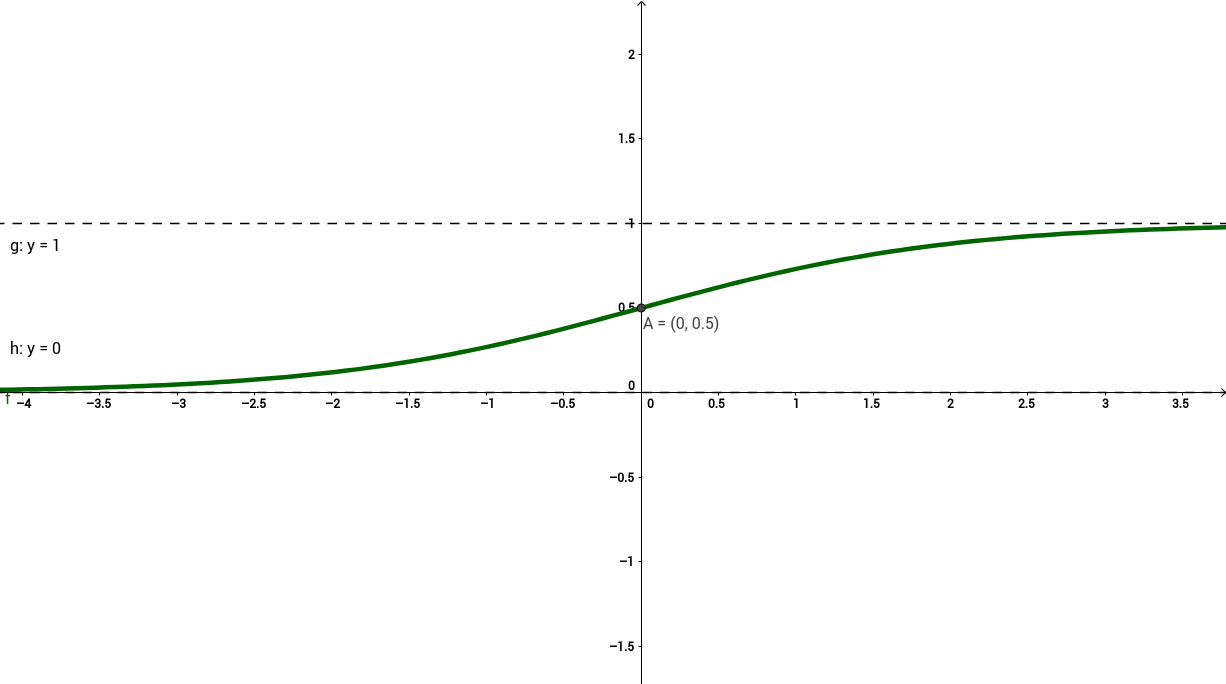
\includegraphics[width=\textwidth]{2017PanelliniesB.png}
        \centering
      \end{figure}
  \end{enumerate}

  \pagebreak[1]
  \section*{Θέμα Γ}
    \begin{enumerate}
      \item [Γ1.] Η εφαπτομένη της γραφικής της $C_f$ στο σημείο $x=x_0$ είναι η

        $$y-f(x_0)=f'(x_0)(x-x_0)$$

        Έχουμε $f(x_0)=-ημx_0$ και $f'(x_0)=-συνx_0$. Έτσι

        $$y+ημx_0=-(x-x_0)συνx_0$$

        Η εφαπτομένη περνάει από το σημείο $Α$ άρα επαληθεύει την εξίσωση, έτσι

        $$-\frac{\pi}{2}+ημx_0=-(\frac{\pi}{2}-x_0)συνx_0 \implies \\\ -\frac{\pi}{2}+ημx_0+(\frac{\pi}{2}-x_0)συνx_0=0$$

        Προφανείς ρίζες είναι οι $x=0$ και $x=\pi$. Θεωρούμε ότι υπάρχει και τρίτη ρίζα στο $(0,\pi)$. Τότε η συνάρτηση $$h(x)=-\frac{\pi}{2}+ημx+(\frac{\pi}{2}-x)συνx$$ θα έχει σύμφωνα με το θεώρημα Rolle 2 ρίζες στην παράγωγό της στο διάστημα $(0,\pi)$. Αλλά $$h'(x)=(x-\frac{\pi}{2})ημx$$ η οποία έχει μοναδική ρίζα στο εν λόγω διάστημα, κάτι το οποίο είναι άτοπο. Έτσι οι δύο προηγούμενες ρίζες είναι και μοναδικές. Για $x=0$ η εφαπτόμενη είναι η $y=-x$ και για $x=\pi$ η εφαπτόμενη είναι η $y=x-\pi$.

      \item [Γ2.] Το εμβαδό $E_2$ είναι ίσο με

        $$\int_{0}^{\pi}-f(x)dx=\int_{0}{\pi}ημxdx=[-συνx]_0^{\pi}=2$$

        Το εμβαδό $E_2$ μπορεί να βρεθεί με την αφαίρεση του εμβαδού του τριγώνου με κορυφές τα $(0,0)$, $(\pi,0)$ και $\left(\frac{\pi}{2},-\frac{\pi}{2}\right)$ με το εμβαδό $E_1$, το οποίο ισούται με $E_2=\frac{\pi\frac{\pi}{2}}{2}-2=\frac{\pi^2}{4}-2$. Έτσι

        $$\frac{E_1}{E_2}=\frac{\frac{\pi^2}{4}-2}{2}=\frac{\pi^2}{8}-1$$

        Η γραφική παράστασή τους είναι

        \begin{figure}[h]
          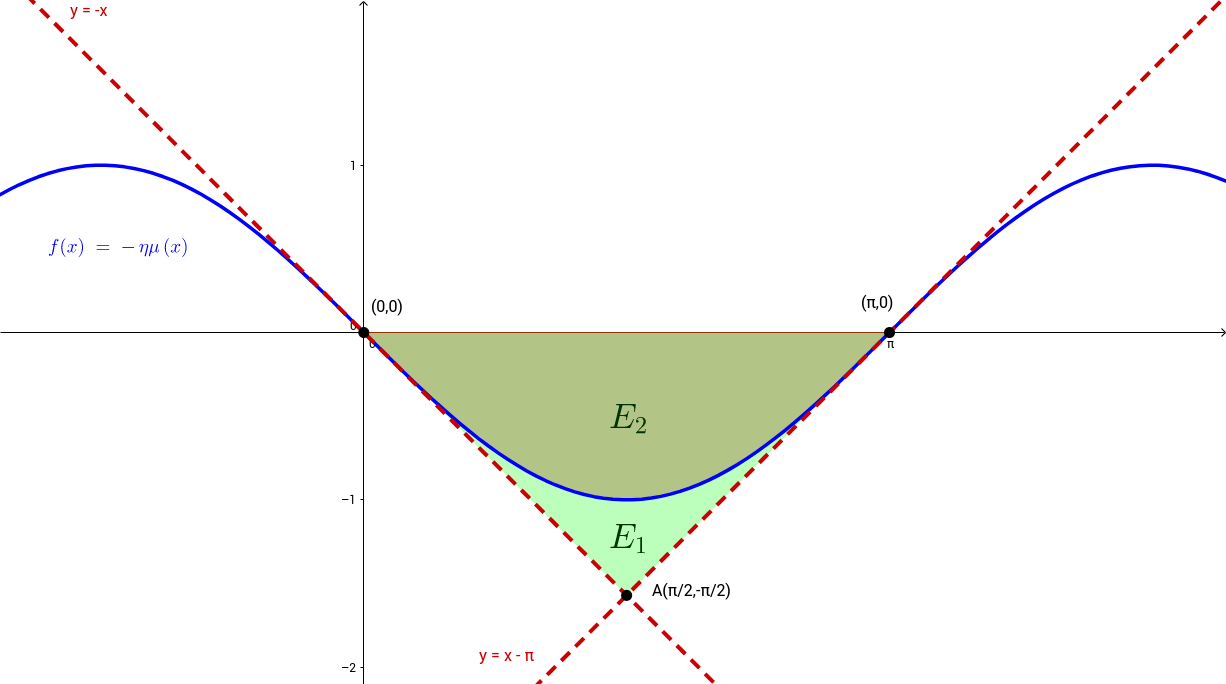
\includegraphics[width=\textwidth]{2017panelliniesΓ.png}
          \centering
        \end{figure}

      \item [Γ3.] Από την γραφική παράσταση έχουμε ότι $f(x)\ge y_{ε_2} \implies f(x)-x+\pi \ge 0$ για κάθε $x\in[0,\pi]$ άρα

      $$\lim_{x\to \pi} \frac{f(x)+x}{f(x)-x+\pi}=\frac{\pi}{0^+}=+\infty$$

      \item [Γ4.] Και πάλι από την γραφική παράσταση, αφού $f(x)> x -\pi$ για κάθε $x\in[1,\pi]$, συνεπώς $\frac{f(x)}{x}> 1-\frac{\pi}{x}$. Έτσι

      $$\int_{1}^{e}\frac{f(x)}{x}dx > \int_{1}^{e}1-\frac{\pi}{x}dx = [x-\pi\ln x]_1^{\pi} = e-1-\pi$$
    \end{enumerate}

    \section*{Θέμα Δ}
      \begin{enumerate}
        \item [Δ1.] Η συνάρτηση σε κάθε της κλάδο είναι συνεχής. Για το σημείο που αλλάζει τύπο έχουμε $\lim_{x\to 0^-}f(x)=0=\lim_{x\to 0^+}f(x)$. Άρα η συνάρτηση είναι συνεχής.

          \begin{itemize}
            \item σημείο που μηδενίζει η παράγωγος:

              $$f'(x)=\begin{cases} -\frac{4}{3}\left(-x\right)^{\frac{1}{3}}, & x\in[-1,0) \\\ e^x(ημx+συνx), & x\in[0,\pi]\end{cases}$$

              Έτσι και μόνο για τον δεύτερο κλάδο, αφού ο πρώτος μηδενίζει μόνο στο $x=0$, έχουμε

              $$e^x(ημx+συνx)=0\implies x=\frac{3\pi}{4}$$

            \item σημεία που δεν ορίζεται η παράγωγος:

              $$\lim_{x\to 0^-}\frac{(-x)^{\frac{4}{3}}-0}{x-0}=0$$

              και

              $$\lim_{x\to 0^+}\frac{e^xημx-0}{x-0}=1$$
          \end{itemize}

Άρα τα κρίσιμα σημεία είναι τα $x=0$ και $x=\frac{3\pi}{4}$.


  \item [Δ2.] Με πίνακα προσήμων για την $f'(x)$ έχουμε

    $$\begin{array}{c | c c c c c c c}
      x & -1 & & 0 & & \frac{3\pi}{4} & & \pi \\ \hline
      -\frac{4}{3}\left(-x\right)^{\frac{1}{3}} & & - & & \cellcolor{blue!25} & \cellcolor{blue!25} & \cellcolor{blue!25}\\
      e^x(ημx+συνx) & \cellcolor{blue!25} & \cellcolor{blue!25} & & + & 0 & - \\ \hline
      f'(x) & & \begin{tikzpicture}[scale=0.5]\draw [->] (0,0) to (1,-0.5);\end{tikzpicture} & & \begin{tikzpicture}[scale=0.5]\draw [->] (0,0) to (1,0.5);\end{tikzpicture} & & \begin{tikzpicture}[scale=0.5]\draw [->] (0,0) to (1,-0.5);\end{tikzpicture}
    \end{array}$$

    άρα η συνάρτηση είναι γνησίως αύξουσα για $x\in(0,\frac{3\pi}{4})$ και γνησίως φθίνουσα για $x\in(-1,0)\cup(\frac{3\pi}{4},\pi)$. Για κάθε ένα από τα διαστήματα βρίσκουμε το σύνολο τιμών και έχουμε

    \begin{equation*}
      \begin{split}
        \left(f(0),f(-1)\right)\cup\left(f(0),f(\frac{3\pi}{4})\right)\cup\left(f(\pi),f(\frac{3\pi}{4})\right)= \\\ \left(0,1\right)\cup\left(0,e^{\frac{3\pi}{4}}\frac{\sqrt{2}}{2}\right)\cup\left(0,e^{\frac{3\pi}{4}}\frac{\sqrt{2}}{2}\right)= \\\
        \left(0,e^{\frac{3\pi}{4}}\frac{\sqrt{2}}{2}\right)
      \end{split}
    \end{equation*}

    Αλλά

    $$e^{\frac{3\pi}{4}}>2 \implies \frac{\sqrt{2}}{2}e^{\frac{3\pi}{4}}>1$$

    άρα το σύνολο τιμών είναι το $f(A)=\displaystyle \left(0,e^{\frac{3\pi}{4}}\frac{\sqrt{2}}{2}\right)$.


    \item [Δ3.] Έχουμε ότι $e^{x}ημx< e^{x}< e^{5x}$ άρα το εμβαδό είναι ίσο με

      $$E=\int_{0}^{\pi}e^{5x}-e^x ημxdx= \\\ \left[\frac{e^{5x}}{5}-\frac{1}{2}e^x (ημx+συνx)\right]_{0}^{\pi}=\frac{e^{5\pi}-1}{5}-\frac{e^\pi}{2}-\frac{1}{2}$$


    \item [Δ4.] Με πολλαπλασιασμό έχουμε

      $$f(x)-\left(\frac{4x-3\pi}{4}\right)^2=e^{\frac{3\pi}{4}}\frac{\sqrt{2}}{2}=f\left(\frac{3\pi}{4}\right) \implies \\\ f(x)-f\left(\frac{3\pi}{4}\right) = \left(\frac{4x-3\pi}{4}\right)^2$$

      Αφού το μέγιστο της συνάρτησης $f$ είναι το $f\left(\frac{3\pi}{4}\right)$, η προηγούμενη εξίσωση ισχύει μόνο για $x=\frac{3\pi}{4}$
    \end{enumerate}


\end{document}
